\documentclass[]{auvsi_doc}
\setkeys{auvsi_doc.cls}{
	AUVSITitle={Design Description},
	AUVSILogoPath={./../logo.pdf}
}

% include extra packages, if needed

\begin{document}

\begin{AUVSITitlePage}
\begin{artifacttable}
\entry{DD-001, 0.1, 04-02-19, Initial release, Derek Knowles, Jacob Willis}
% additional \entry{} commands for extra rows in the revision table, if needed
\end{artifacttable}
\end{AUVSITitlePage}

% document contents (see below for LaTex commands that make your life easier)
\section{Introduction}
% Appropriate (brief) background of the project. Indicate why the project is important. Share your project objective statement. Indicate the key success measures for the project.

The BYU AUVSI Capstone team is competing in the AUVSI-SUAS 2019 competition this summer. The mission portion of the competition requires a small unmanned aircraft system (UAS) to autonomously fly to given waypoints, avoid imaginary obstacles, identify visual and geospatial characteristics of objects on the ground, and accurately drop a payload consisting of an unmanned ground vehicle (UGV) that is capable of autonomously driving to another location. Our team consists of four primary subteams: Airframe, Controls, Vision, and UGV. This artifact will summarize the description of each subteam.

\section{Design Description}
% Briefly describe the design in words and with appropriate top-level pictures. The description should not be a detailed definition. The detailed definition is found in the artifacts. The description should provide an overview of the design that will make it easy for the reader to understand the details found in the artifacts. Refer to appropriate design artifacts as needed.
A summary of each subteam's design description is provided in the subsections below.

\subsection{Airframe}

The airframe subteam selected the Nimbus Pro airframe. It is a fixed-wing plane with a large storage capacity and large wing span made of polystyrene (Fig. \ref{fig:plane1}). It was selected during Concept Development for its long span and spacious fuselage. Multiple flight tests have been performed with
R/C control and the autopilot. We have also successfully tested system integration with the UGV drop and vision subsystems during flight.

\begin{figure}[h!]
	\centering
	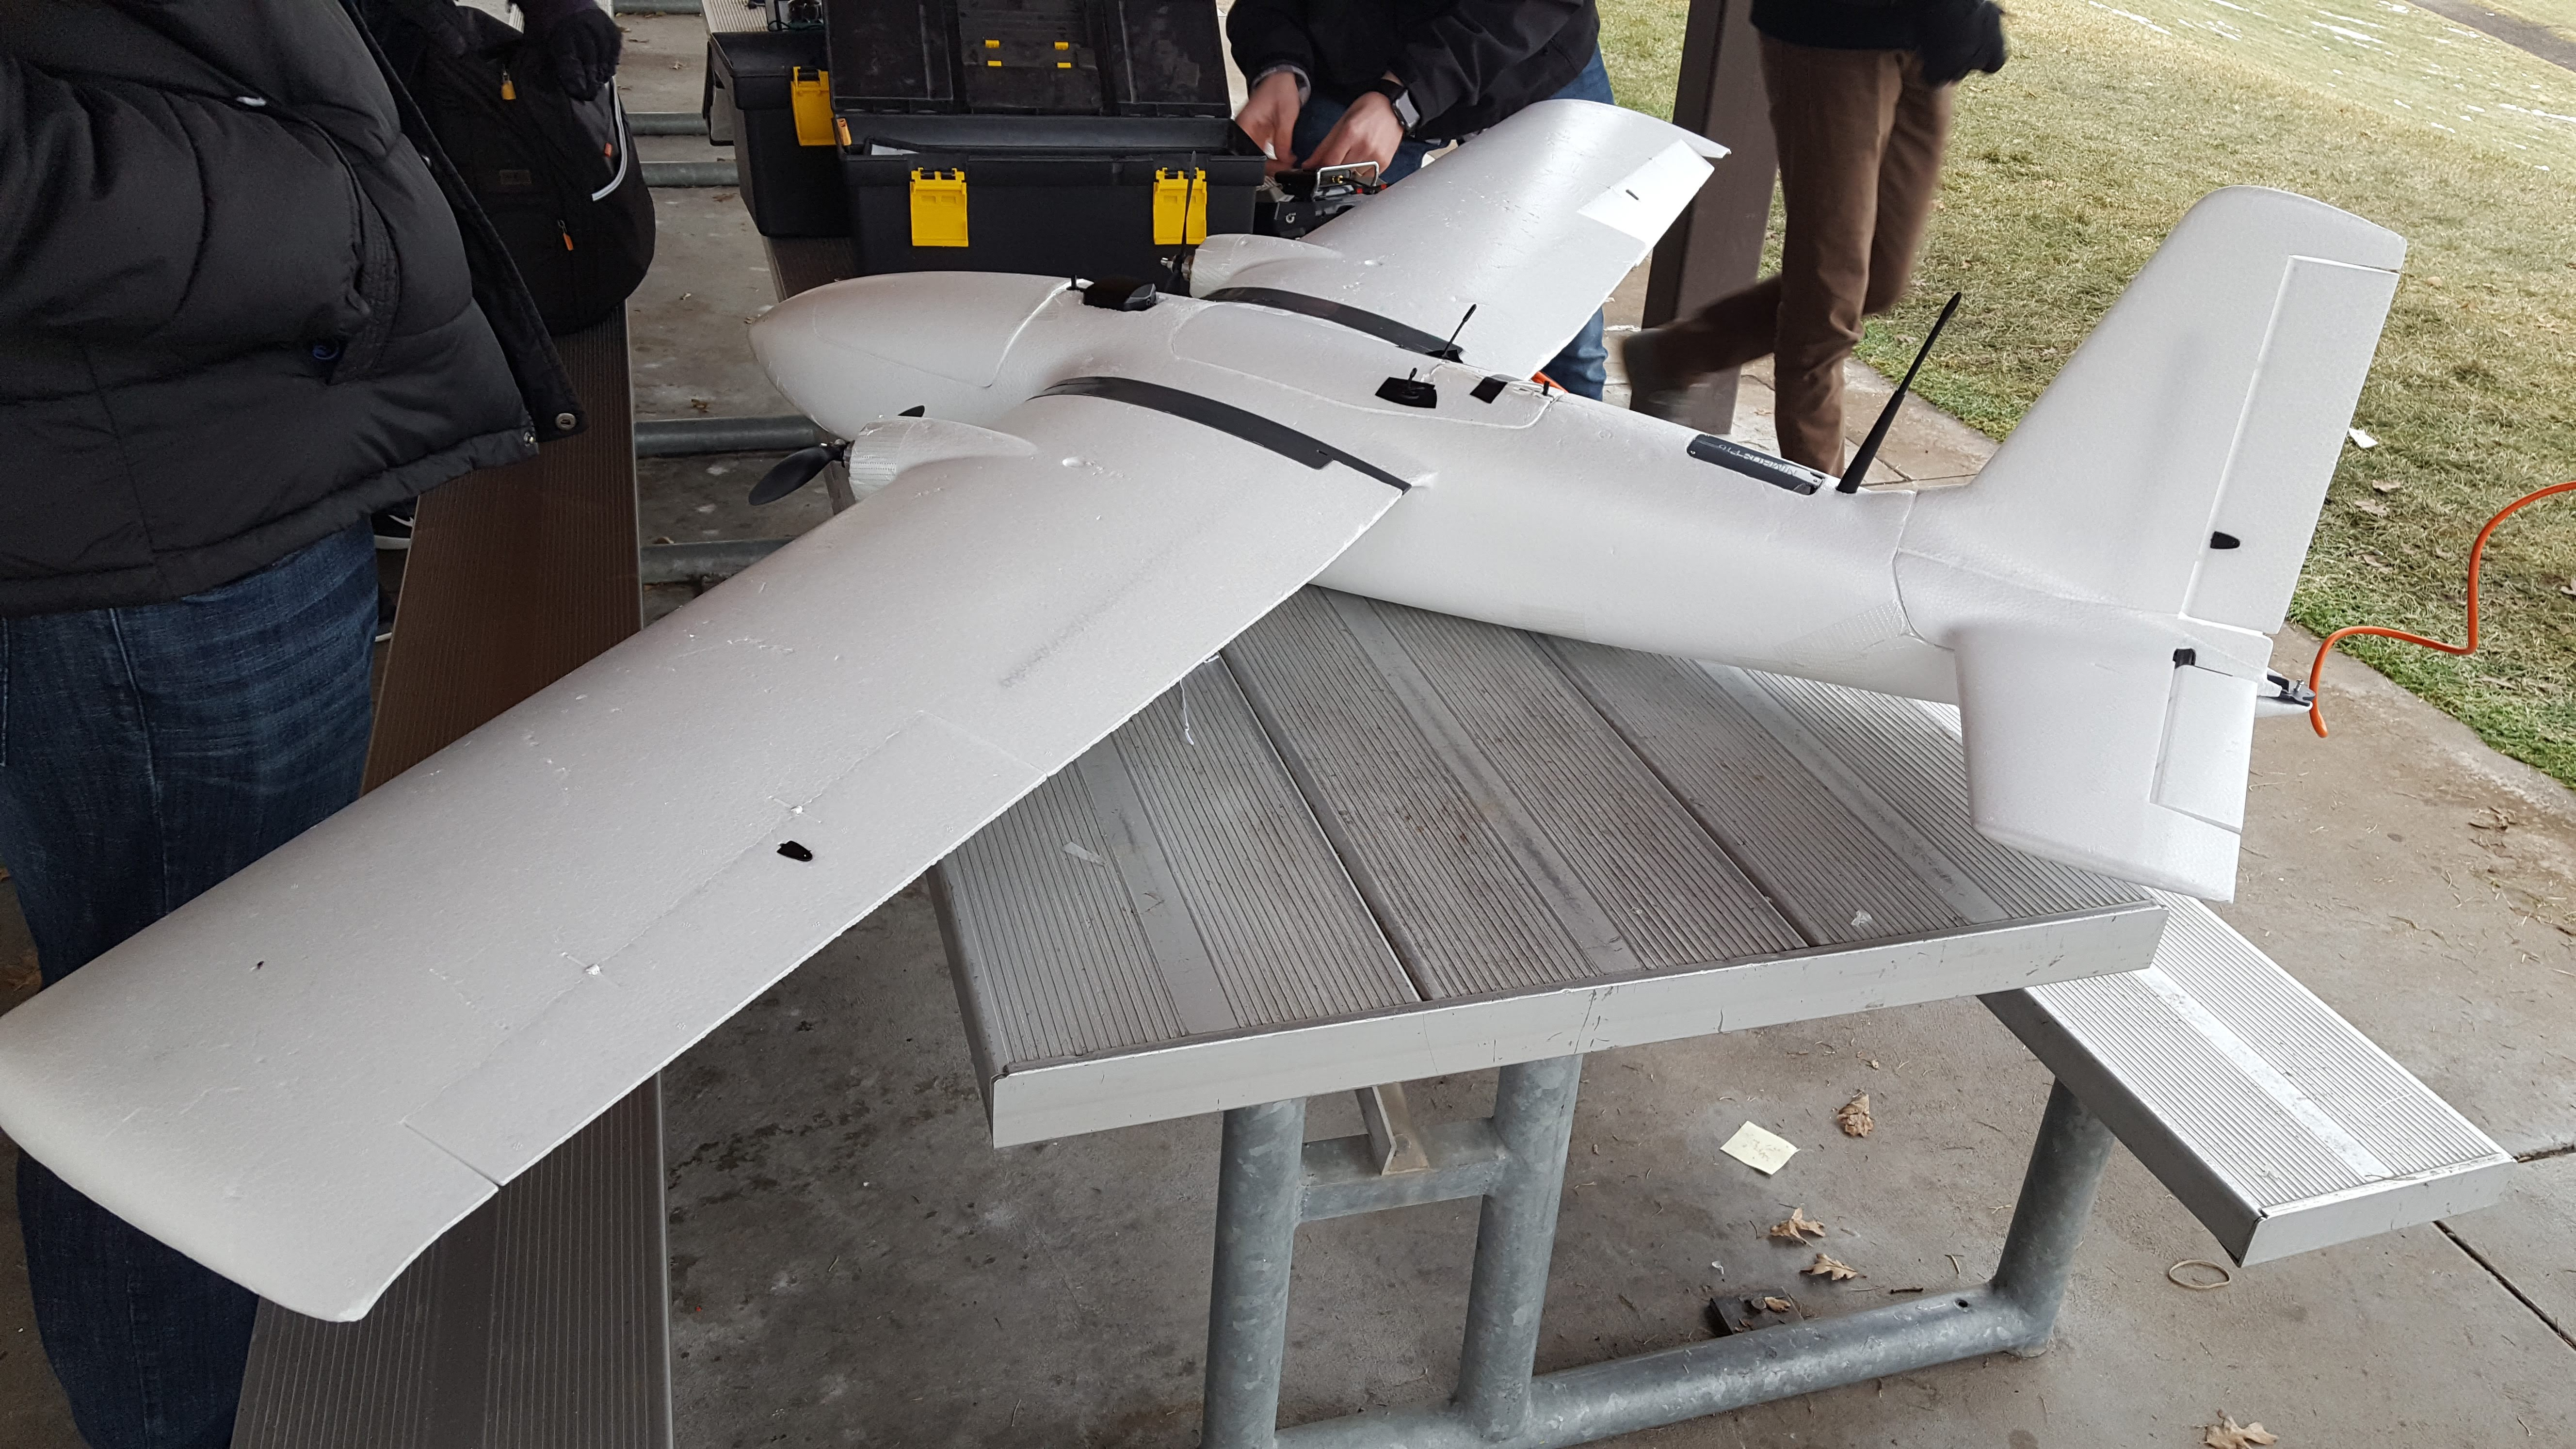
\includegraphics[width=.9\columnwidth]{figs/plane1}
	\caption{Fully-constructed Nimbus Pro airframe before its first flight.}
	\label{fig:plane1}
\end{figure}

\subsection{Controls}


\subsection{Vision}

In order to address concerns with the way the past year's team spread information
across multiple machines making it difficult to identify bugs, replicate
results and setup quickly, our team created a
basic server-client architecture as defined as shown in Figure \ref{fig:serverFlow}.

\AUVSIFigure
{./figs/serverFlowchart.pdf}
{\textwidth}
{Server Architecture}
{fig:serverFlow}

The basic data flow of all these components is shown in Figure \ref{fig:dataFlow}.

\AUVSIFigure
{./figs/basicDataFlow.pdf}
{\textwidth}
{AUVSI Imaging Data Flow Through Autonomous/Manual Classification}
{fig:dataFlow}

Data flows back and forth between client and server, with the server holding a definitive-final
copy of a target image, as well as a history of its state during intermediate steps.

\subsection{UGV}

The UGV is to be loaded within the aircraft. Upon a command from the flight controller system, a small hatch opens and the UGV falls out. The UGV is carried to the ground by a lightweight 36 inch nylon parachute, purchased from FruityChutes. The parachute is loaded onto the aircraft in a tube that allows the UGV to pull it out of the aircraft as it falls. This helps stop the tangling that can come from a folded parachute. To also prevent tangling, and to make for a more predictable drop, the parachute is folding according to GV-007. After exiting the aircraft the parachute will be opened by drag. This will slow down the system enough to allow the UGV to survive impact without damage. A visual depiction of our chosen system can be seen in Fig.~\ref{fig:side}.

\begin{figure}[h]
\centering
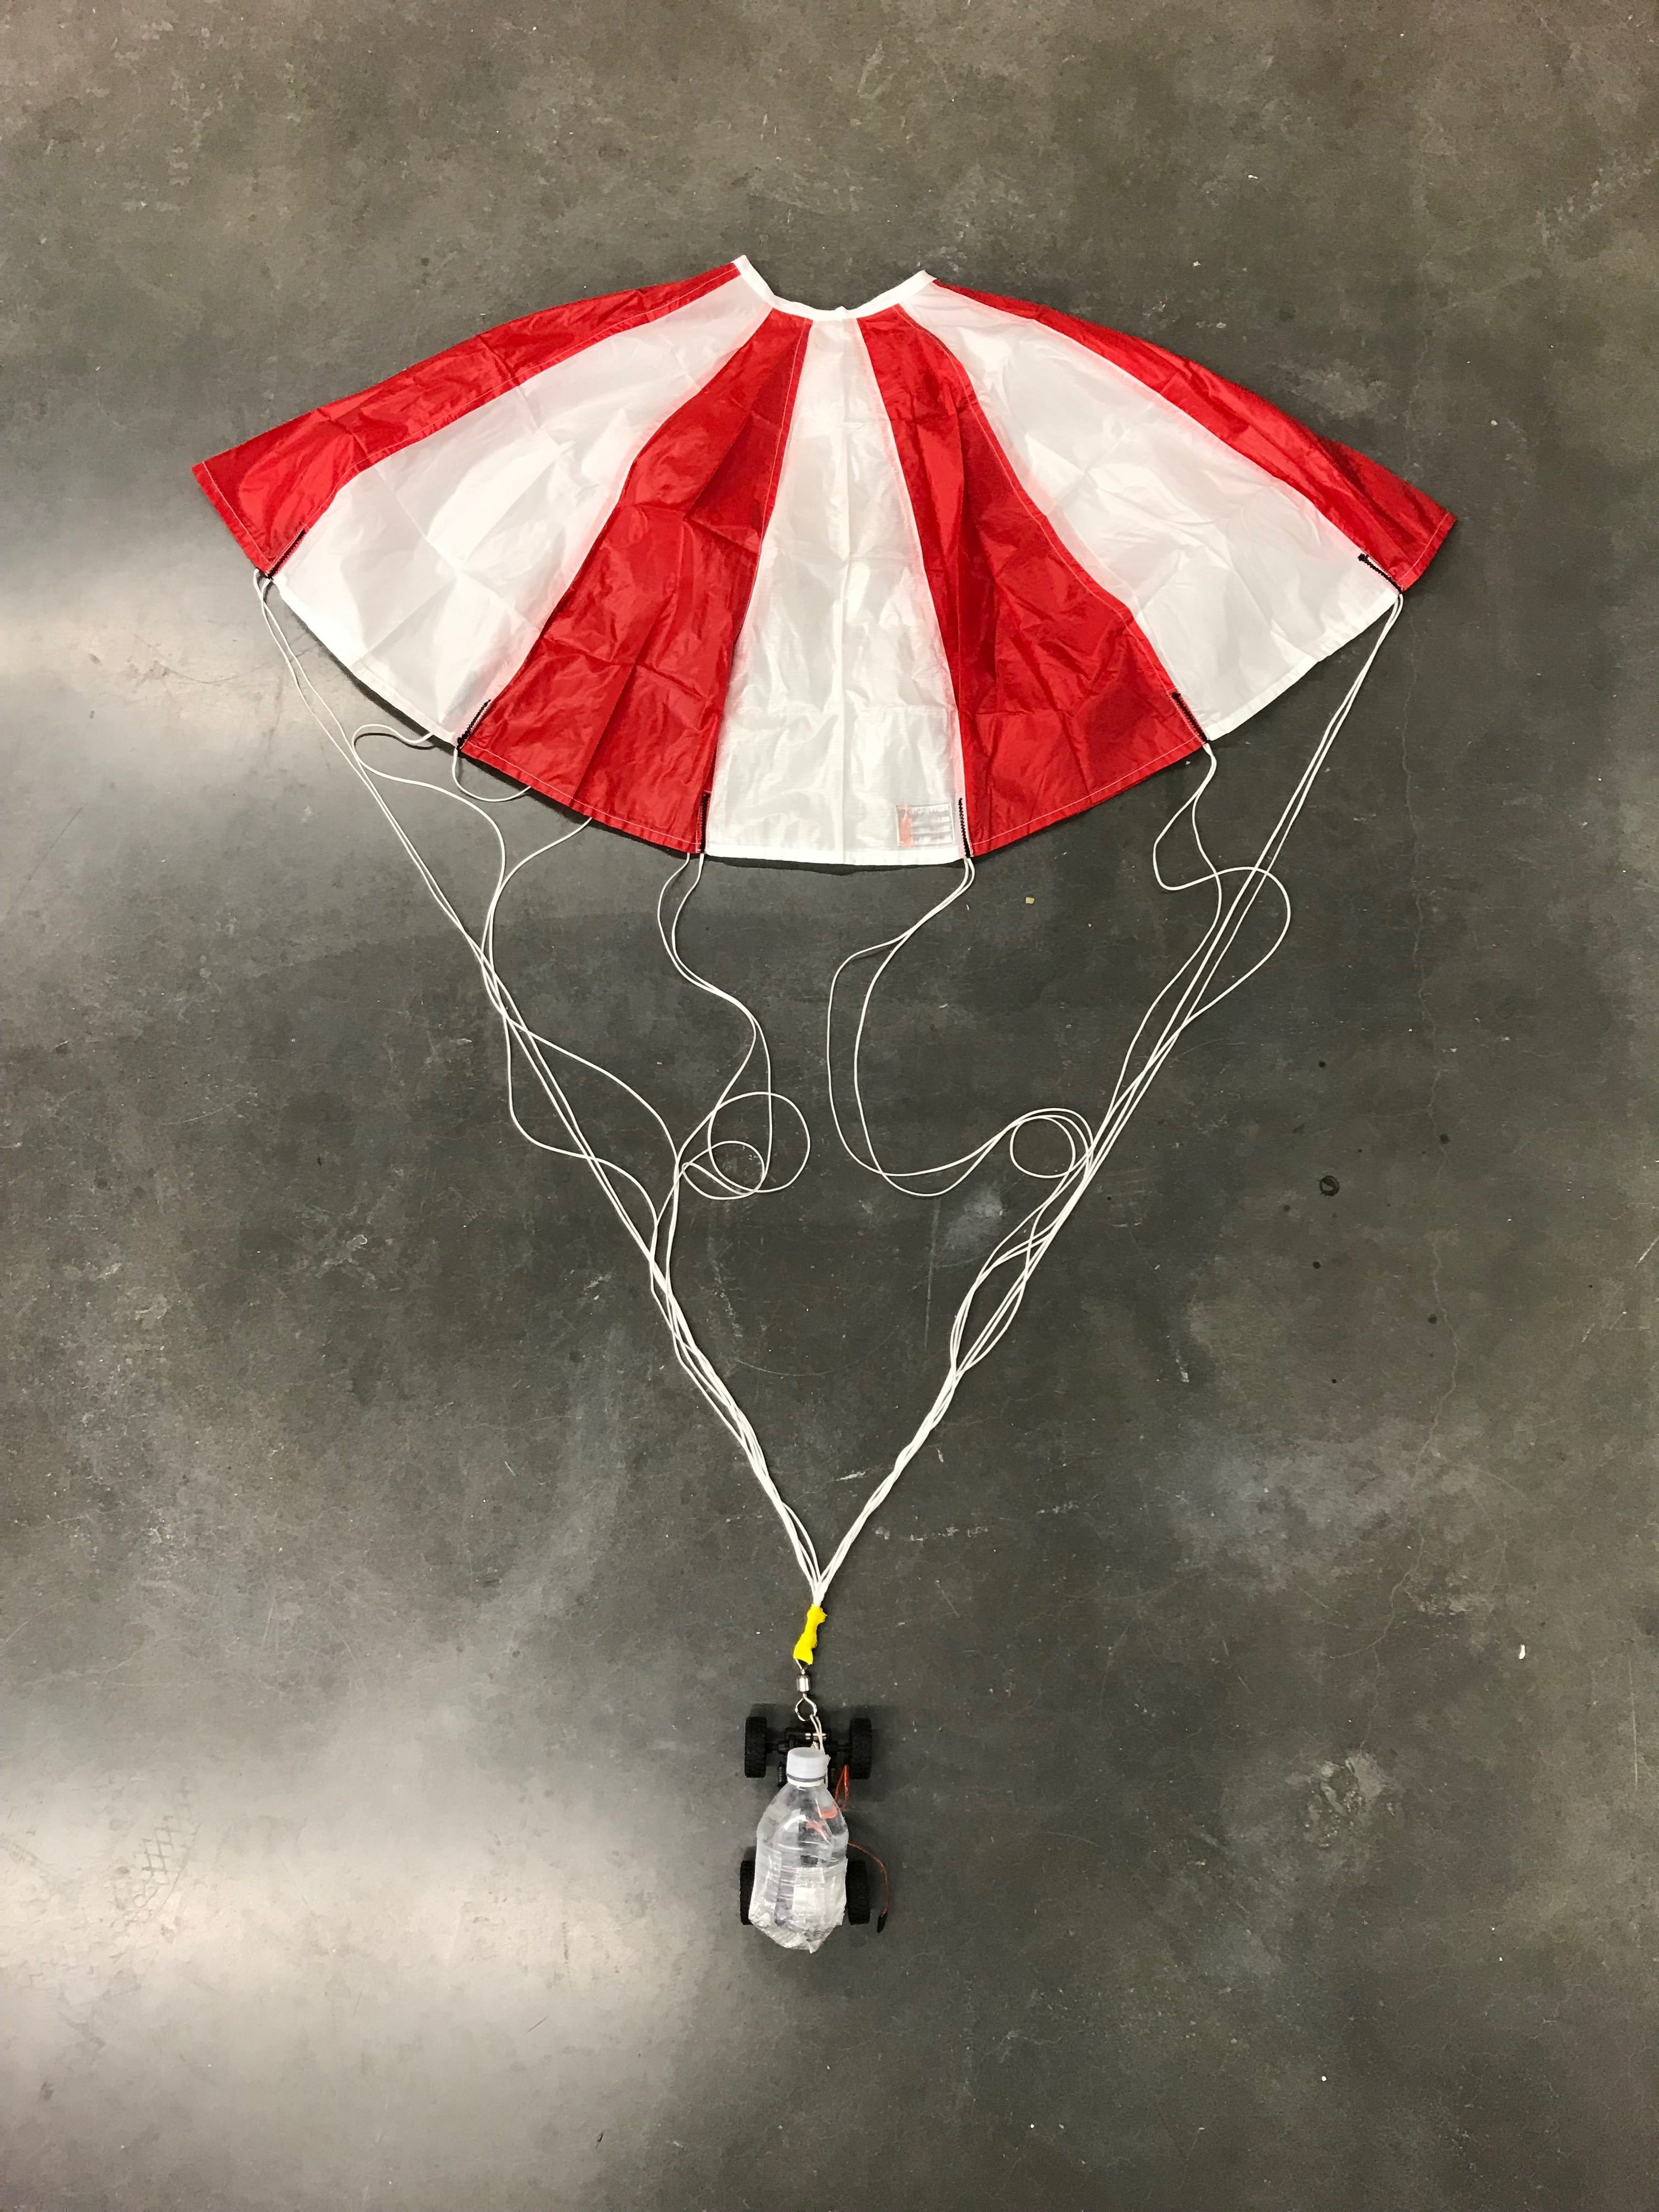
\includegraphics[width=90mm]{./figs/Parachute_Side.jpg}
\caption{Our parachute and simulated UGV as seen from the side.}
\label{fig:side}
\end{figure}

\section{Conclusion}

This year's AUVSI team has increased the desirability and transferability of the Unmanned Aircraft System. Each subteam
has make progress on each of the key success measures thereby increasing the reliability of each subsystem.

\end{document}
